
\chapter{Deep Learning Approach}

\label{Chapter4}

%----------------------------------------------------------------------------------------

In the previous chapters we have introduced the key components of the approach we followed in our study: on the one hand, we have described existing satellite image datasets and introduced the actual data we will consider, and on the other, we have discussed Deep Learning, how it works and how we can use it for our problem. Now, we are ready to describe our approach, the image feature extraction, the model architecture and the training scenario.

\section{Image features and transfer learning}\label{sec:transferLearning}

In order to train a model based on images, some sort of features need to be extracted. Traditionally, this image feature extraction was based on a set of hand-crafted detectors aimed to detect edges, corners, blobs and other feature descriptors. Some of these detectors are the Sobel filter, Laplacian of Gaussian (LoG), Difference of Gaussians (DoG), Determinant of Hessian (DoH), SIFT \parencite{Lowe1999,Lowe2004}, SURF \parencite{Bay2006}, Histograms of Oriented Gradients (HOG) \parencite{Dalal2005} and Gabor filters.

\begin{figure}[h!]
	\centering
	\begin{subfigure}{.5\textwidth}
  		\centering
  		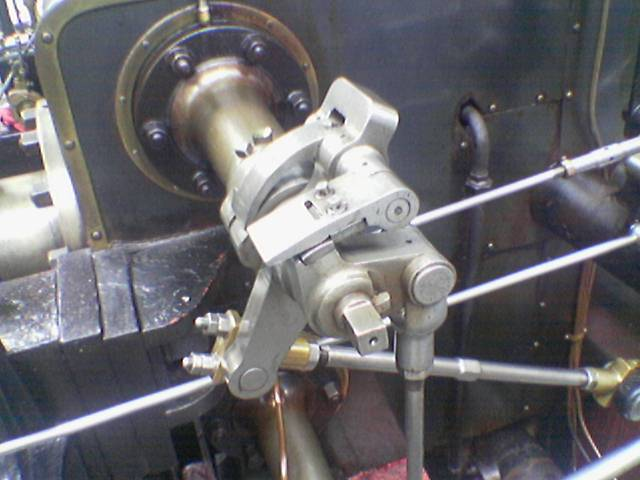
\includegraphics[width=.9\linewidth]{sobel_valve_original.png}
	\end{subfigure}%
	\begin{subfigure}{.5\textwidth}
  		\centering
  		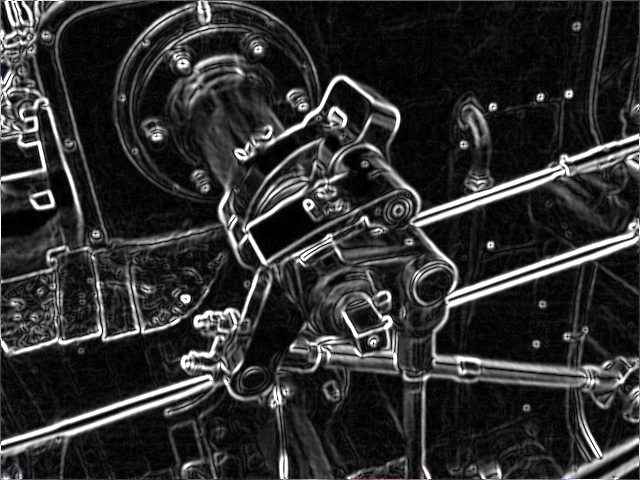
\includegraphics[width=.9\linewidth]{sobel_valve_processed.png}
	\end{subfigure}
	\captionsetup{width=1\linewidth}
	\caption{\textbf{Example of the Sobel filter}}
	\label{fig:sobel}
\end{figure}

\begin{figure}[h!]
	\centering
	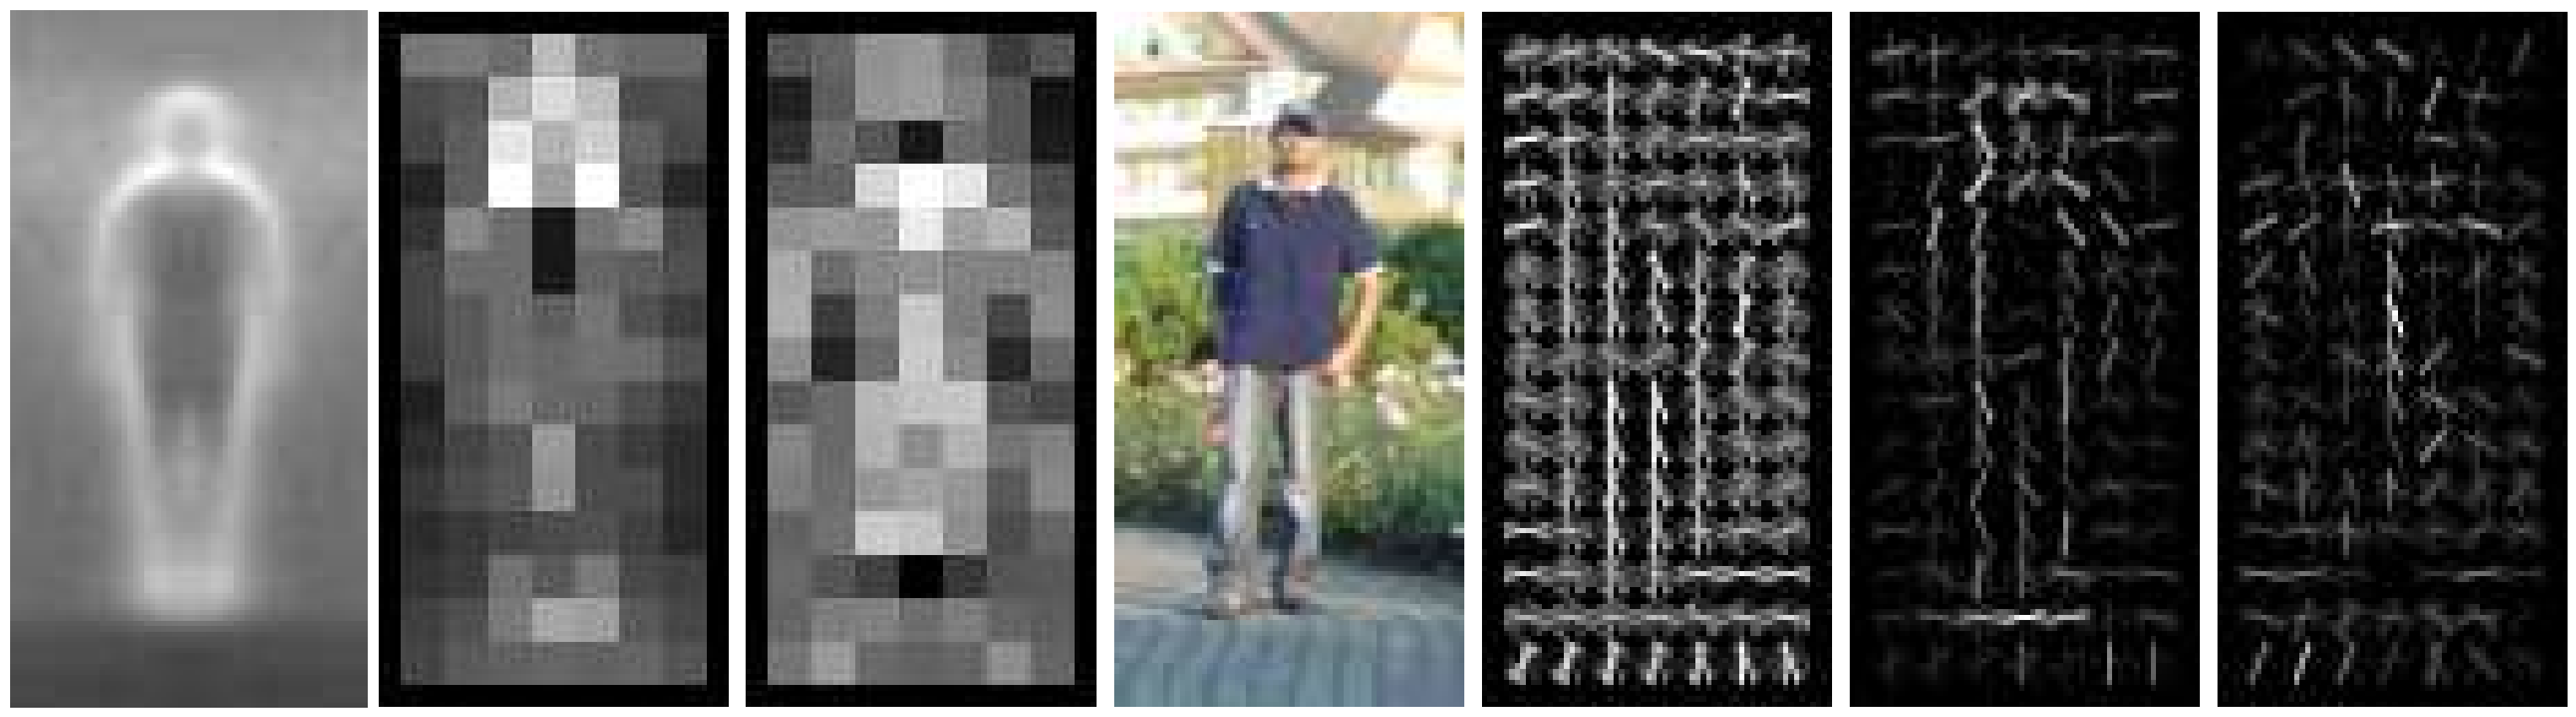
\includegraphics[width=0.9\textwidth]{Figures/hog_example.png}
	\captionsetup{width=1\linewidth}
	\caption{\textbf{Examples of HOG detector \parencite{Dalal2005}}}
	\label{fig:hog}
\end{figure}

More recent approaches to image classification using Neural Networks have benefited from the existing and increasing computational power, and deep Convolutional Neural Networks have been able to achieve higher performances than traditional models. 

Yet, training a deep CNN from scratch for a particular problem requires a large and exhaustive dataset along with a huge amount of computational power. However, it has been shown that the architectures of pre-trained NN can be reused for other purposes and achieve an equally great performance. This is known as \textbf{Transfer Learning}. Figure \ref{fig:transfer_learning_idea} schematizes this idea.

\begin{figure}[h!]
	\centering
	\captionsetup{width=1\linewidth}
	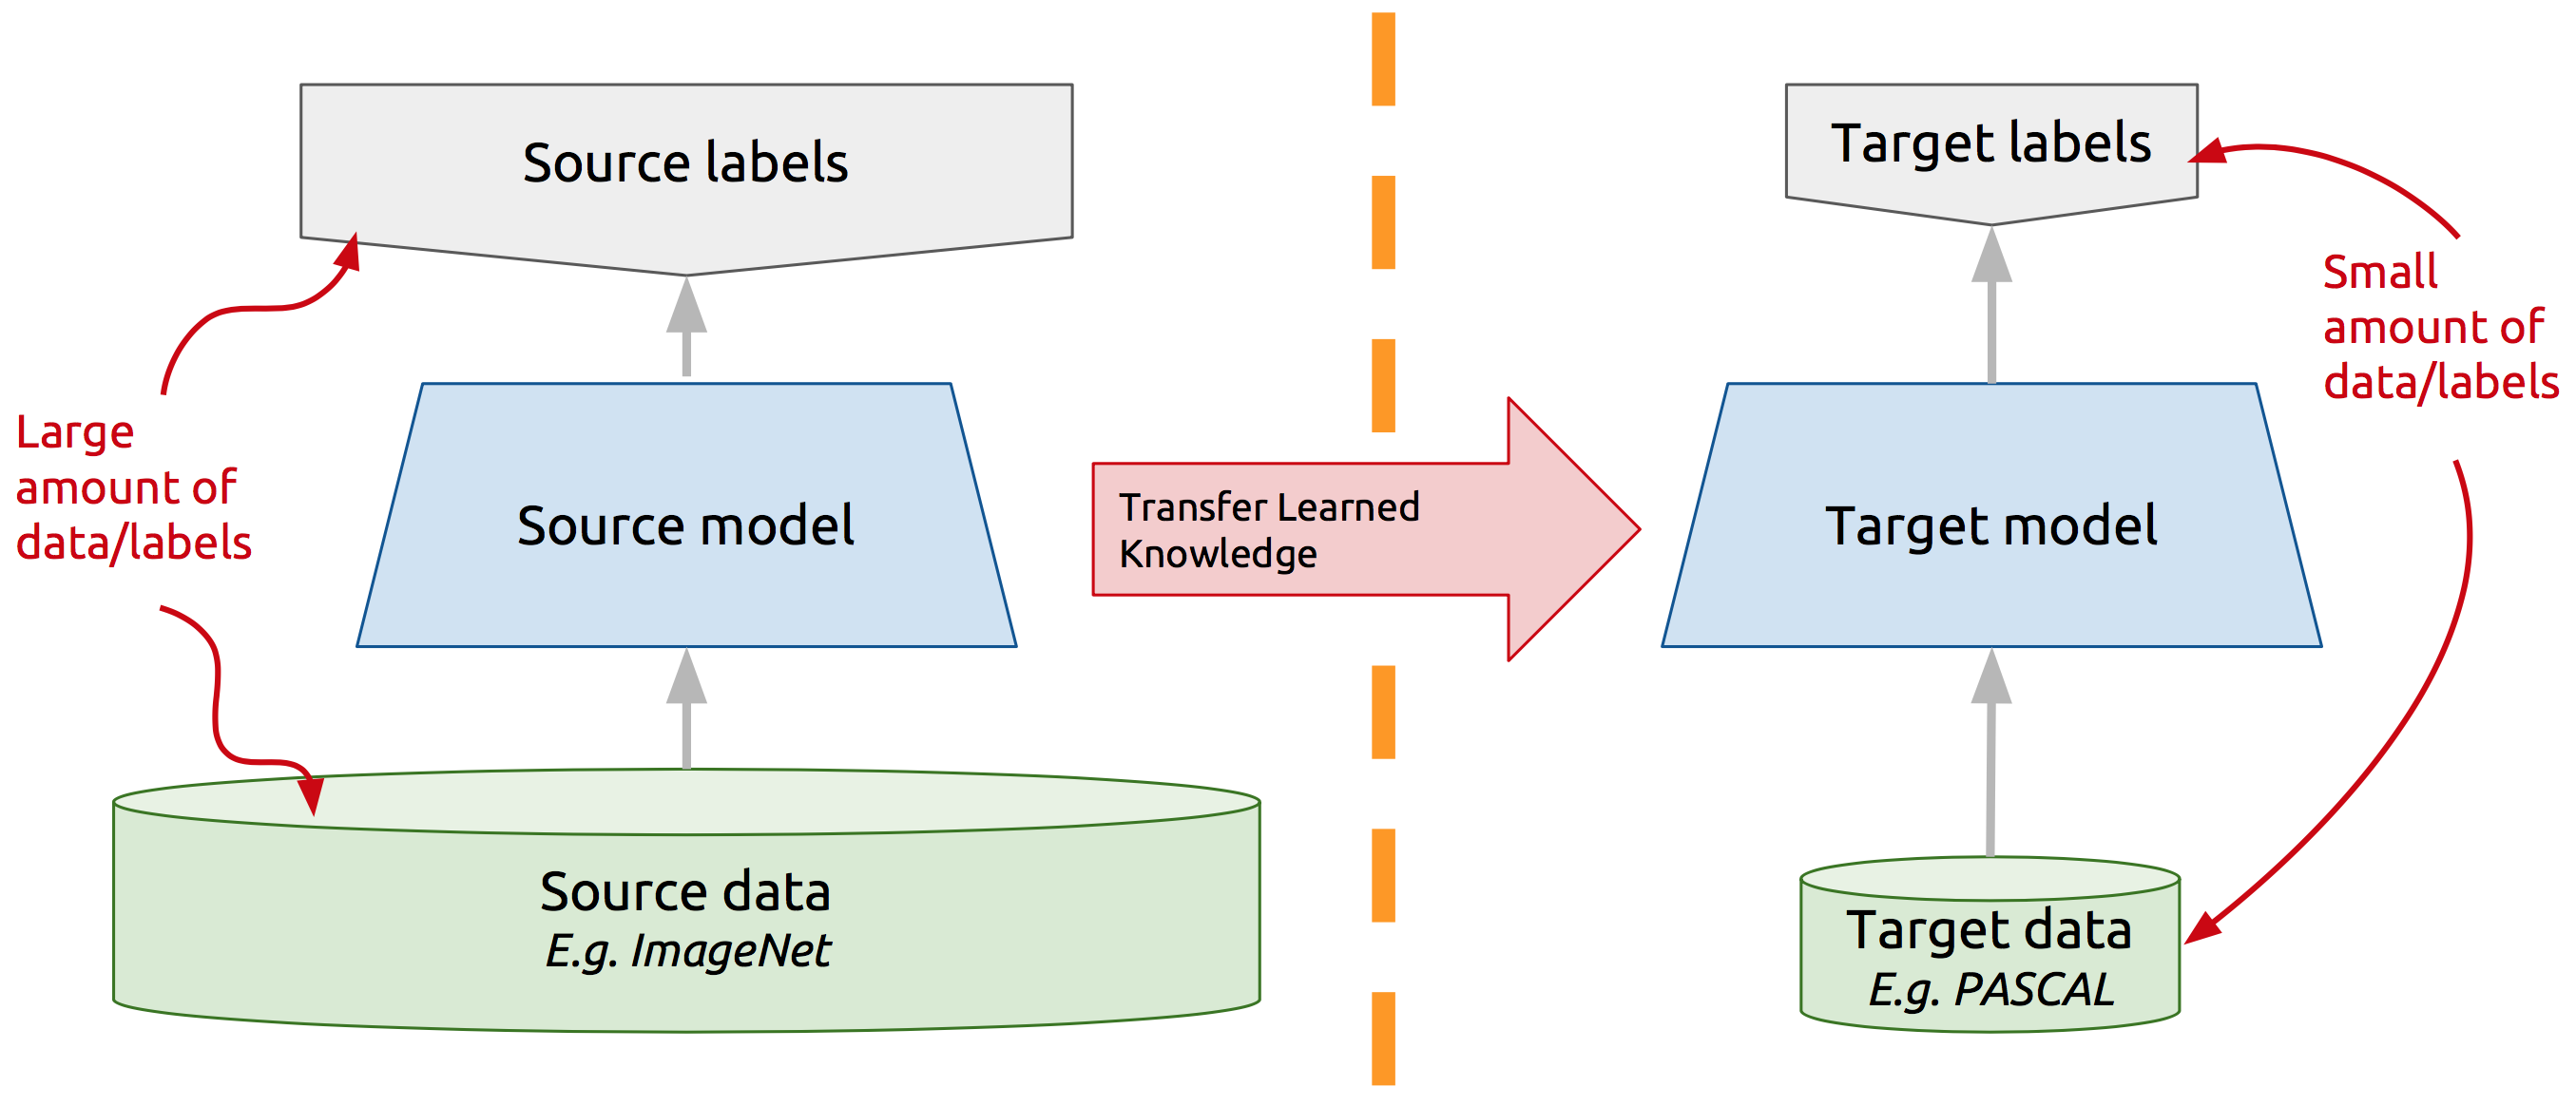
\includegraphics[width=1\textwidth]{Figures/transfer_learning_idea.png}
	\caption{\textbf{Transfer Learning}: a model learned from a large dataset can be transferred and reused for another purpose. \parencite{McGuinness2017}}
	\label{fig:transfer_learning_idea}
\end{figure}

These pre-trained architectures can be re-purposed by reusing the learned weights and either replacing the final layers of the net by some other classifier, or even fine-tuning all the layers for the specific problem. In any case, the initial layers of the Neural Network provide a great image feature extractor.

\

In the next section we describe our approach using transfer learning from a ResNet architecture.

%Consequently, there is an increasing library of available pre-trained models and weights: Xception, VGG, InceptionV3, ResNet.
%Most of these models have weights pre-trained on ImageNet, a large dataset containing more than 14 million hand-annotated images and over 20.000 categories.

%\begin{figure}[h!]
%	\centering
%	\captionsetup{width=1\linewidth}
%	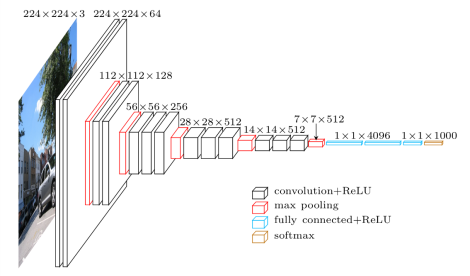
\includegraphics[width=1\textwidth]{Figures/imagenet_vgg16.png}
%	\caption{\textbf{VGG16 architecture}. Stack of $3\times 3$ convolutional and max pooling layers.}
%	\label{fig:degrade}
%\end{figure}

%\subsection{ResNets}

%Experience with Neural Networks, and CNN in particular, show that deeper nets tend to perform better, as these are more capable to model higher complexity. Yet, at some depth point, training becomes too difficult, because the gradient values obtained from the loss function are lost after several layers. This is known as \textbf{vanishing gradient}. ResNet fixes this is issue with Residual...

\section{Proposed architecture}\label{sec:dl_architecture}

As described before (Sections \ref{sec:CNNArchitectures} and \ref{sec:transferLearning}), we can use for our problem a pre-trained ResNet with our own final classification layers. Hence, the architecture we propose for our problem consists on the activation layers of the ResNet, which act as the feature extractors of our images, followed by a shallow classifier made of a single Dense (Fully Connected) layer. Figure \ref{fig:transfer_learning} gives a schema of this approach.

\begin{figure}[h!]
	\centering
	\captionsetup{width=1\linewidth}
	\includegraphics[width=1\textwidth]{Figures/transfer_learning.png}
	\caption{\textbf{Transfer Learning from a ResNet} (figure adapted from \parencite{McGuinness2017})}
	\label{fig:transfer_learning}
\end{figure}

\subsection{ResNet activations}

The ResNet we consider (ResNet50) has a total of $49$ activation layers, so the output at each of them is different. Initial layers are able to recognize edges, textures and patterns while keeping and image size similar to the input. On the other hand, deeper activation layers show more convoluted relations and provide much more channels (or filters) by shrinking the image size.

For instance, for an input image of (tensor) size $512 \times 512 \times 3$ (a $512x512$ image with $3$ RGB channels), the output of the first activation layer is of size $256 \times 256 \times 64$, the $10^{th}$ gives a $128 \times 128 \times 256$ tensor, and the last $49^{th}$ activation layer outputs $16 \times 16 \times 2048$. For our purpose, we will consider the final output of the ResNet ($49^{th}$ activation layer), although this could be further investigated and discussed.

\

Figures \ref{fig:act_agriculture}, \ref{fig:act_forest_woodland}, \ref{fig:act_shrubland_grassland} and \ref{fig:act_semi_desert} show some outputs of the $10^{th}$ and $49^{th}$ activation layers for samples of different categories in the dataset. Some of the $10^{th}$ activations are particularly sensitive to edges, shadows, or textures, which later translate into different outputs of $49^{th}$ layer.

\begin{figure}[h!]
	\centering
	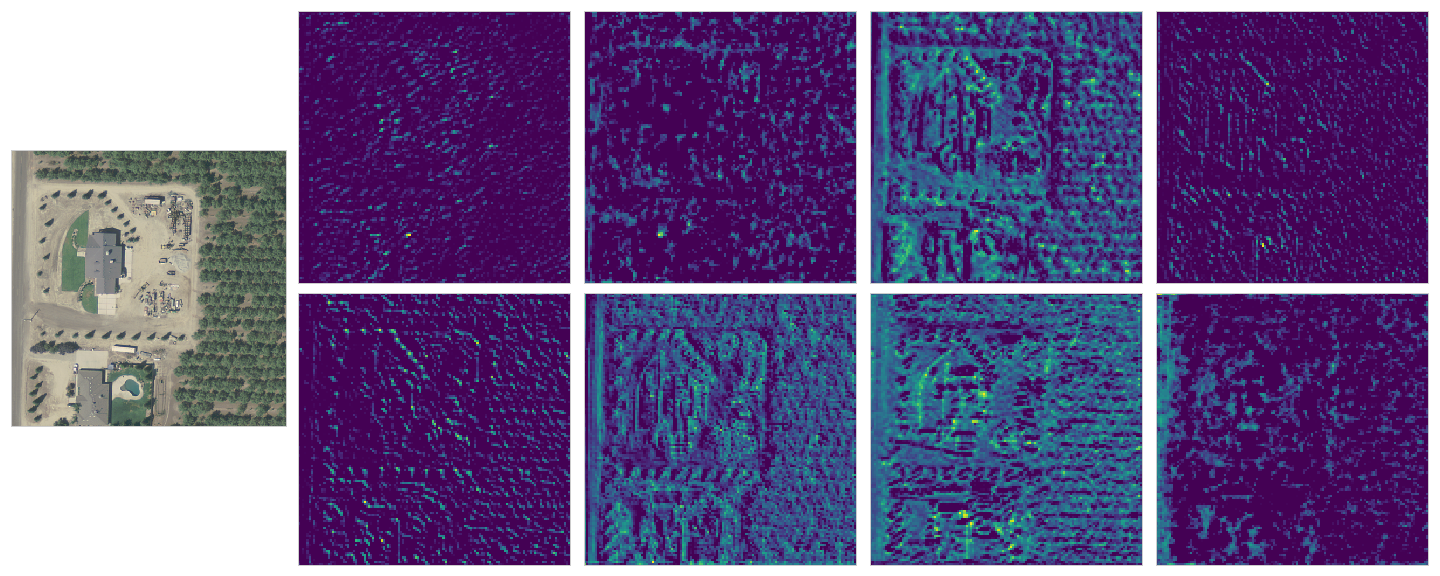
\includegraphics[width=0.9\textwidth]{Figures/activations/agriculture_l2_s1_activation_10.png}
	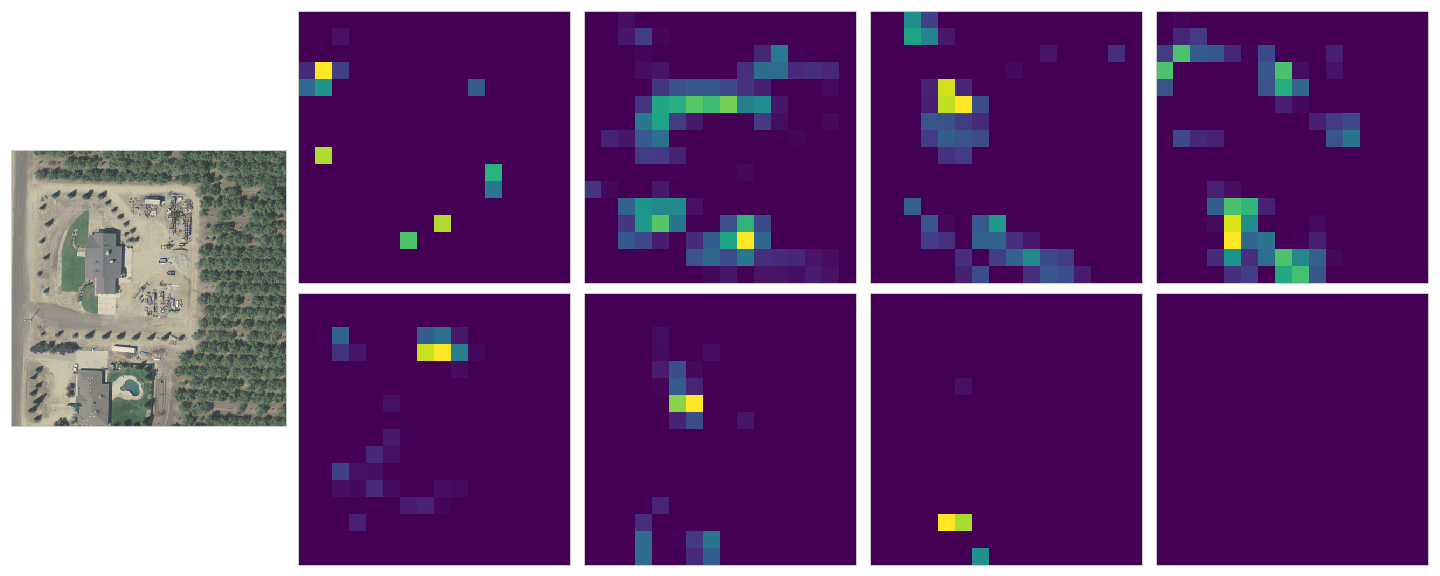
\includegraphics[width=0.9\textwidth]{Figures/activations/agriculture_l2_s1_activation_49.png}
	\captionsetup{width=1\linewidth}
	\caption{\textbf{ResNet activations of an Agriculture image: $10^{th}$ layer (top) and final layer, $49^{th}$ (bottom).}}
	\label{fig:act_agriculture}
\end{figure}

\begin{figure}[h!]
	\centering
	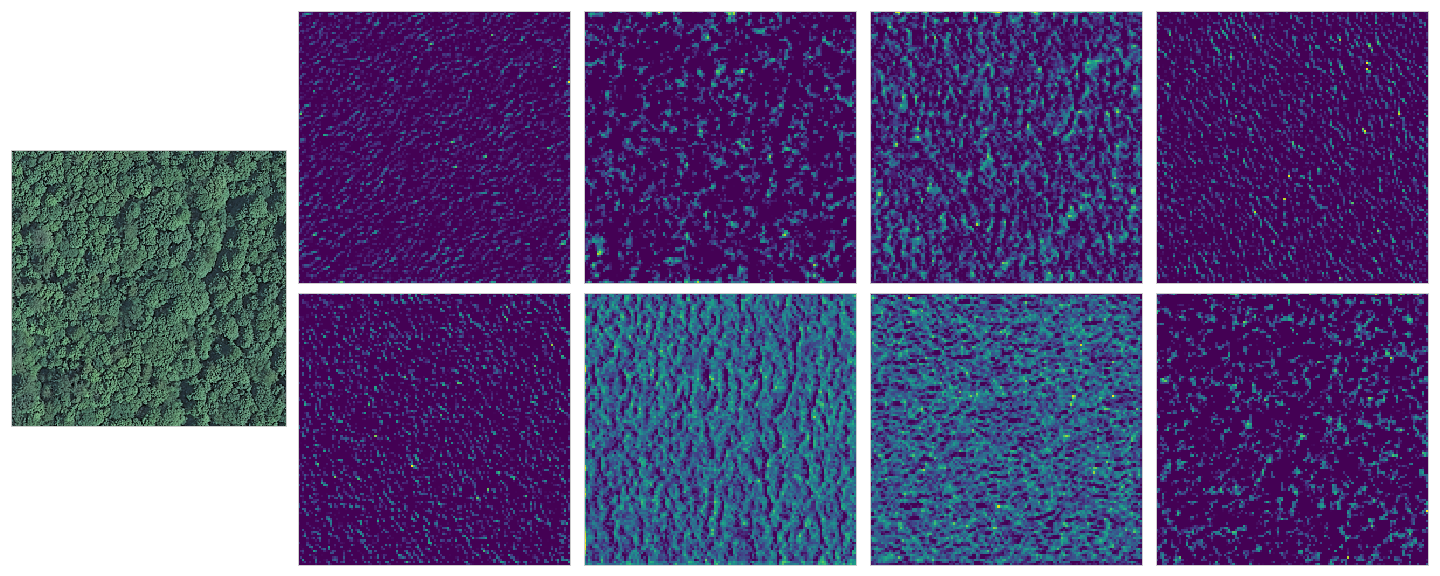
\includegraphics[width=0.9\textwidth]{Figures/activations/forest-woodland_l0_s1_activation_10.png}
	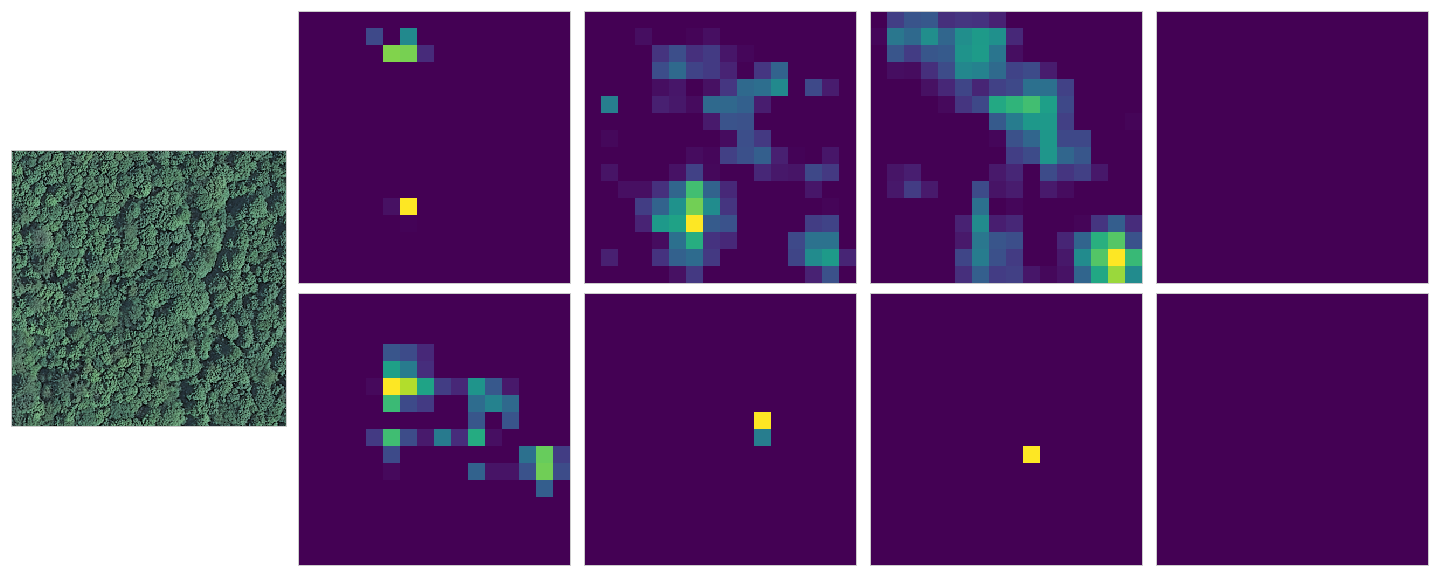
\includegraphics[width=0.9\textwidth]{Figures/activations/forest-woodland_l0_s1_activation_49.png}
	\captionsetup{width=1\linewidth}
	\caption{\textbf{ResNet activations of a Forest-woodland image: $10^{th}$ layer (top) and final layer, $49^{th}$ (bottom).}}
	\label{fig:act_forest_woodland}
\end{figure}

\begin{figure}[h!]
	\centering
	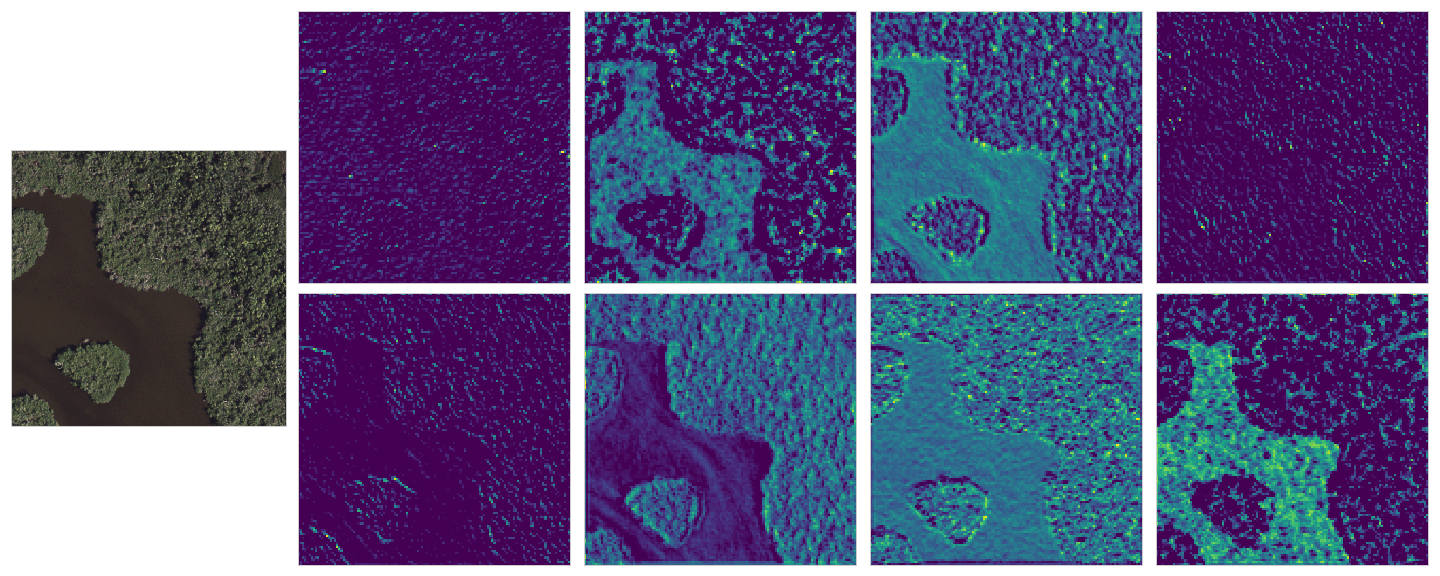
\includegraphics[width=0.9\textwidth]{Figures/activations/shrubland-grassland_l0_s1_activation_10.png}
	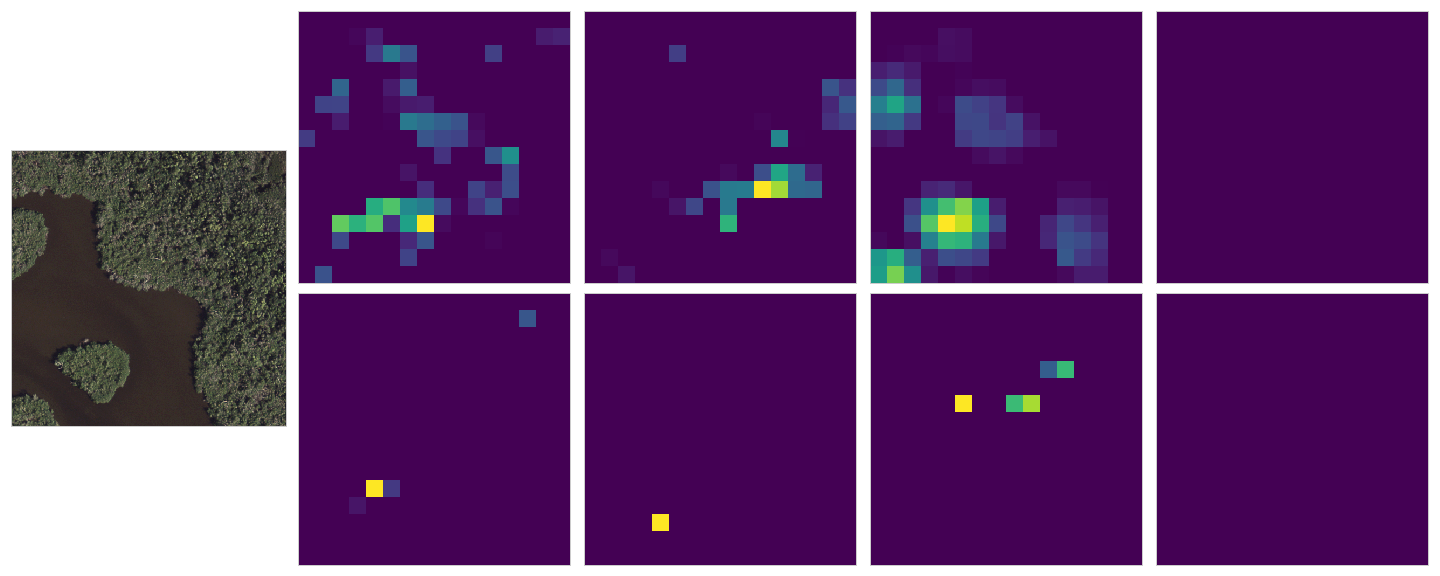
\includegraphics[width=0.9\textwidth]{Figures/activations/shrubland-grassland_l0_s1_activation_49.png}
	\captionsetup{width=1\linewidth}
	\caption{\textbf{ResNet activations of a Shrubland-grassland image: $10^{th}$ layer (top) and final layer, $49^{th}$ (bottom).}}
	\label{fig:act_shrubland_grassland}
\end{figure}

\begin{figure}[h!]
	\centering
	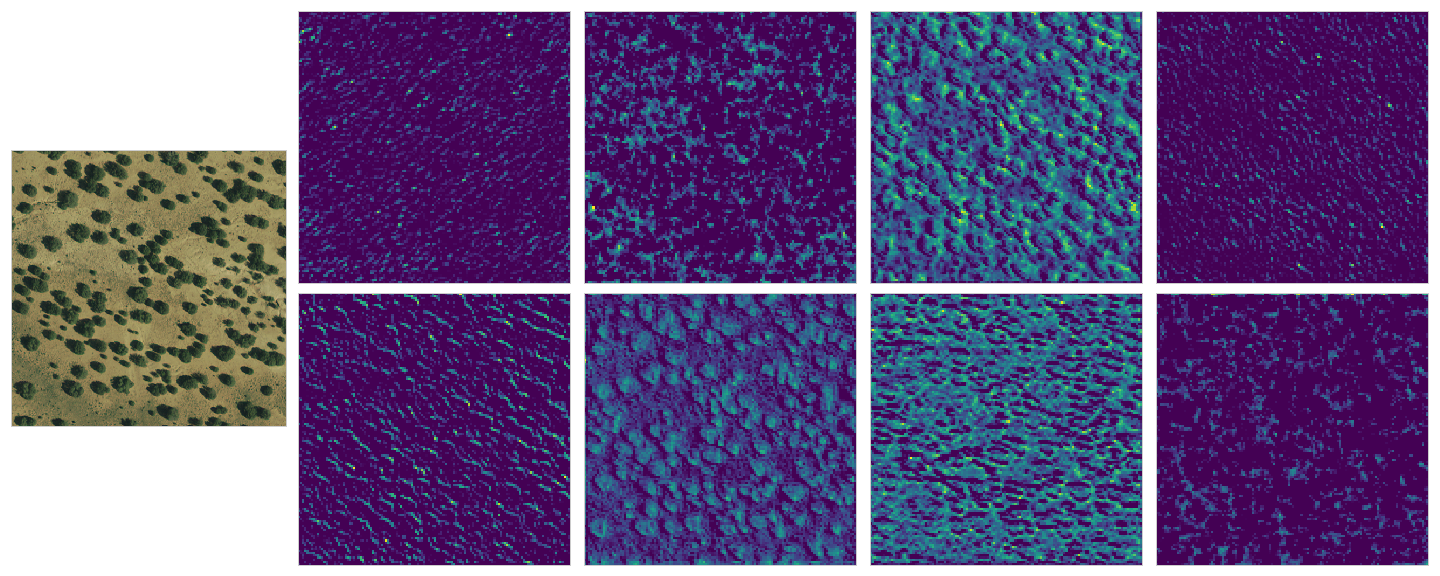
\includegraphics[width=0.9\textwidth]{Figures/activations/semi-desert_l0_s1_activation_10.png}
	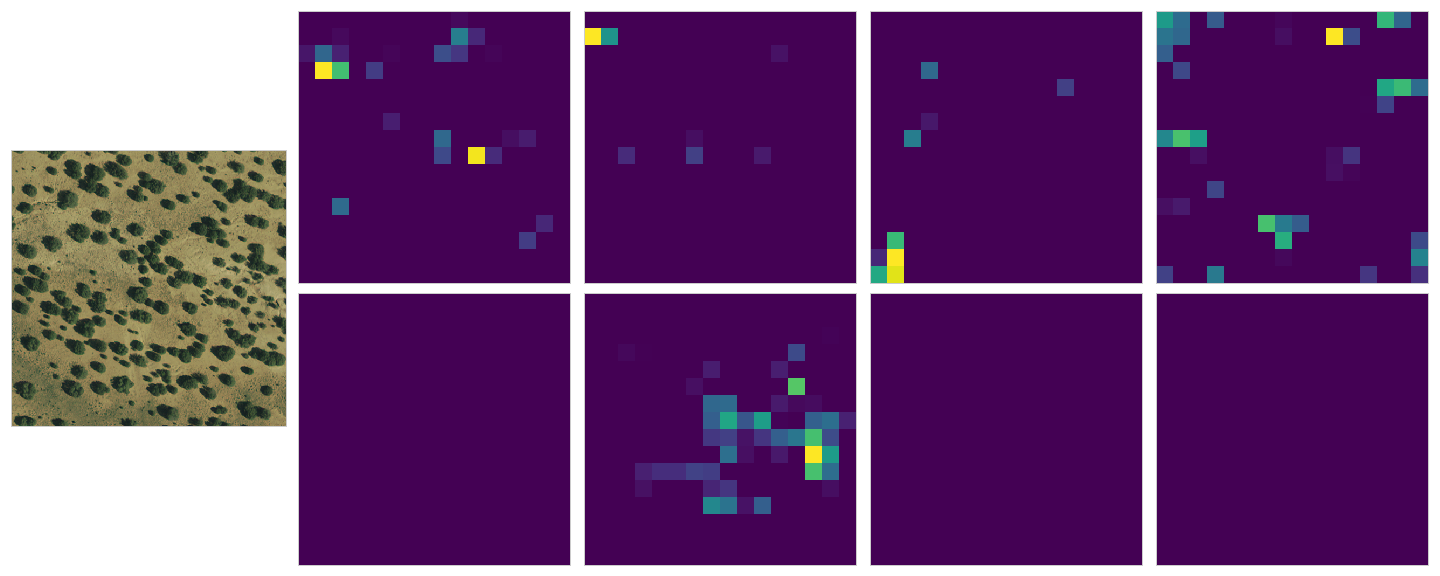
\includegraphics[width=0.9\textwidth]{Figures/activations/semi-desert_l0_s1_activation_49.png}
	\captionsetup{width=1\linewidth}
	\caption{\textbf{ResNet activations of a Semi-desert image: $10^{th}$ layer (top) and final layer, $49^{th}$ (bottom).}}
	\label{fig:act_semi_desert}
\end{figure}

\subsection{Complete architecture}

As mentioned before, for our purpose we considered the last ($49^{th}$) activation layer of the ResNet as the features of our images. These features can be extracted and saved on disk in order to speed up the process (as we did), or computed each time, and then passed through a simple Neural Network.

Then, our model consisted on a single dense layer of $100$ or $512$ neurons \textcolor{red}{(CHECK)} with ReLU activation, followed by a single Dense node with a Sigmoid activation acting as the classifier. This model is then trained on the dataset with and RMSprop optimizer and a binary cross-entropy loss function. This same architecture is then used and trained separately for each of the resolutions considered.

\

All this architecture (see Fig. \ref{fig:transfer_learning}) has been implemented with Python and Keras. Figure \ref{fig:model_keras} shows the model build, and in the following section we describe the complete pipeline with more detail.

\begin{figure}[h!]
	\centering
	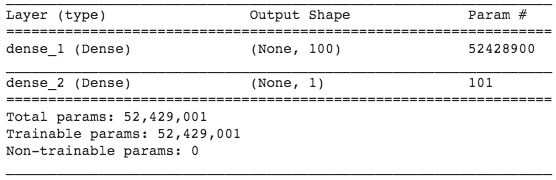
\includegraphics[width=0.7\textwidth]{Figures/model_keras.png}
	\captionsetup{width=1\linewidth}
	\caption{\textbf{Model build with Keras}}
	\label{fig:model_keras}
\end{figure}

\subsection{Training and experiments}

In order to perform the experiments, we consider the following pipeline for each of the datasets ($0.3m$ and $1m$ resolution):

\begin{enumerate}
	\item Load the original images (at the original resolution) from disk.
	\item Downsample the images to the desired resolution.
	\item Compute the ResNet activations (at the $49^{th}$ activation layer) of the resulting images (and save to disk for later use).
	\item Consider a stratified KFold split of the dataset (with $8$ splits) for cross-validation. That means, the dataset is split into $8$ sets with labels $0-1$ equally distributed.  
	\item Train the model separately for each combination of $7$ train sets, with the remaining one as validation. Then results of the $8$ experiments are averaged for more consistency.
	\item Repeat for all downgraded resolutions needed.
\end{enumerate}

Further experiments in order to fine-tune the model complexity and the splitting parameters could be done, but it is not the goal of this project.

\textcolor{red}{RE-DO PLOTS: accuracy-loss per epoch averaged with k-folds?}

%Run models:
%- for both datasets
%- check number of neurons (100, 512?)
%- change plot colors of categories to fixed
%- 

\begin{figure}[h!]
	\centering
	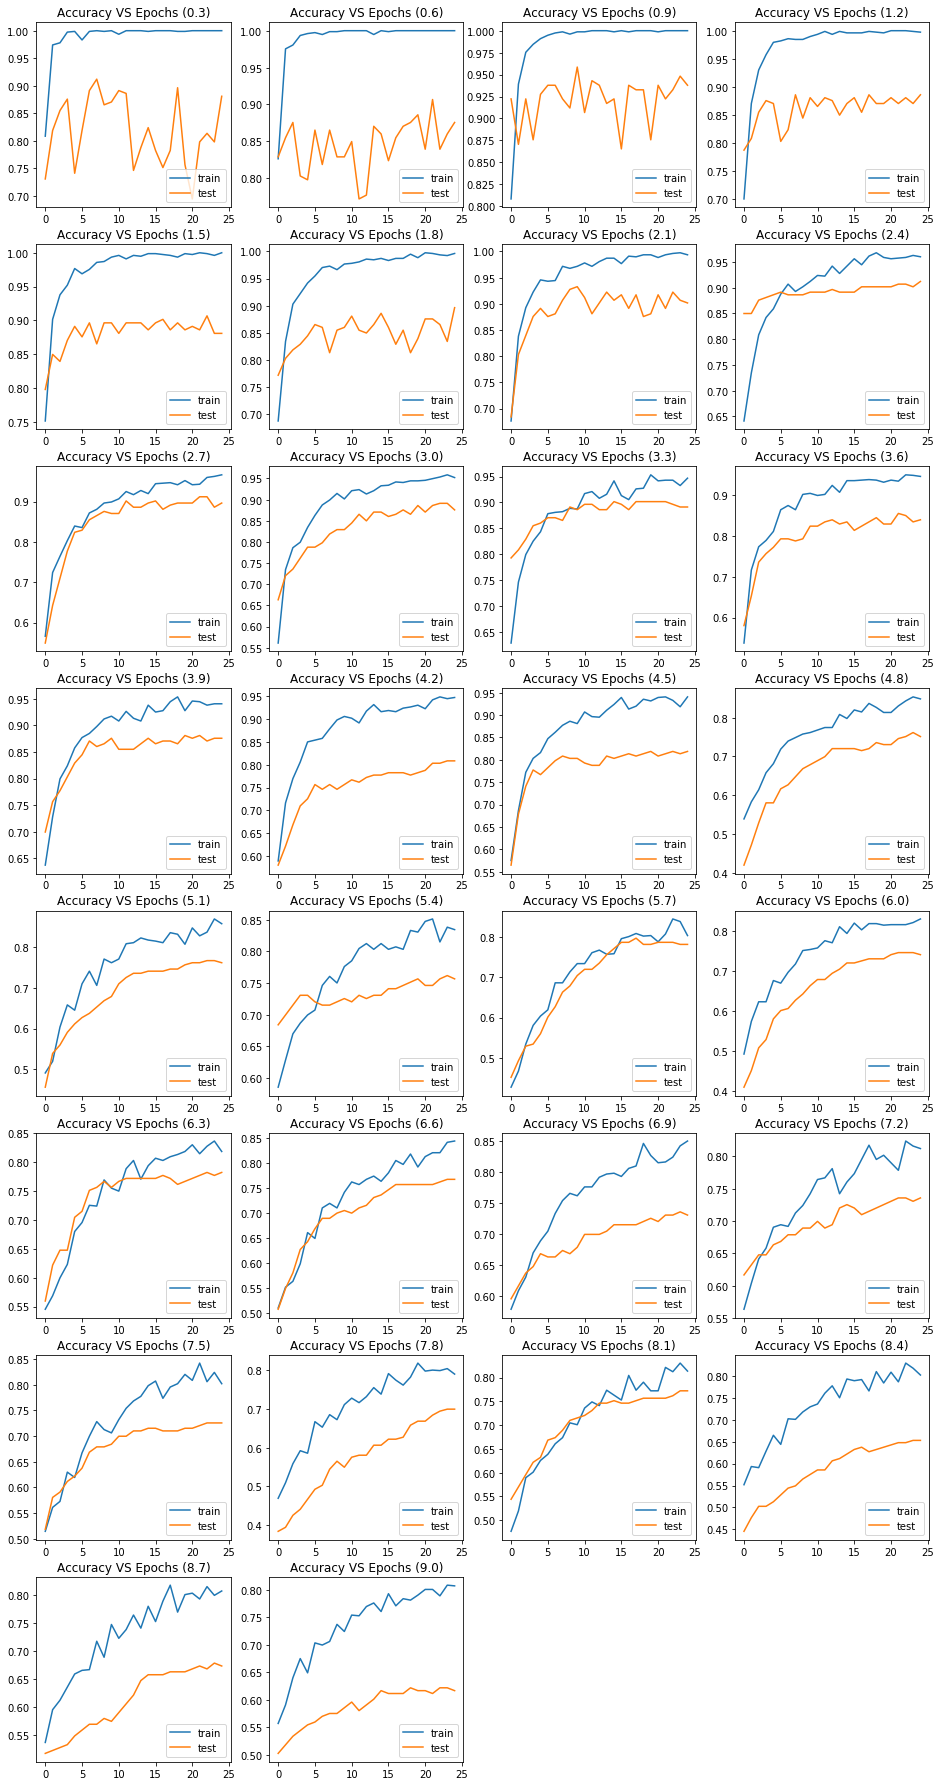
\includegraphics[width=0.9\textwidth]{Figures/convergence_plots_all_res.png}
	\captionsetup{width=1\linewidth}
	\caption{\textbf{Convergence plots for all downgraded resolutions of the $0.3m$ dataset.}}
	\label{fig:conv_plots}
\end{figure}



Transfer learning: 

\begin{itemize}
	\item VGG: \url{https://arxiv.org/abs/1409.1556}
	\item \url{https://iopscience.iop.org/article/10.1088/1742-6596/1087/6/062032/pdf}
	\item \url{https://arxiv.org/abs/1805.02294}
	\item \url{https://cs.nyu.edu/~fergus/papers/zeilerECCV2014.pdf}
	\item \url{https://towardsdatascience.com/transfer-learning-from-pre-trained-models-f2393f124751}
	\item \url{https://www.mitpressjournals.org/doi/pdf/10.1162/neco_a_00990}
	\item \url{https://towardsdatascience.com/a-comprehensive-hands-on-guide-to-transfer-learning-with-real-world-applications-in-deep-learning-212bf3b2f27a}
\end{itemize}